\section{Appendix for Chapter 2}

\subsection{Solve regularized weighted least squares with cyclic coordinate descent}
\label{a.1}
To solve regularized weighted least squares, equation \eqref{eq2.9}, we first compute the gradient at current estimates of $(\tilde{\bm{\gamma}}, \tilde{\bm{\alpha}})$. Let $\gamma_j$ be the $j^{th}$ coordinate of $\bm{\gamma}$, $1\leq j\leq p$; $\alpha_k$ be the $k^{th}$ coordinate of $\bm{\alpha}$, $1\leq k\leq q$. The gradient of equation \ref{eq2.9} with respect to $\gamma_j$ is 
\begin{displaymath}
-\frac{1}{n} \sum_{i=1}^n w_ix_{ij}(y'_i-\bm{\gamma}^T\bm{x}_i-\bm{\alpha}^T(
\bm{xz})_i) + \lambda_1\gamma_j.
\end{displaymath}
Setting the gradient with respect to $\gamma_j$ to 0, the coordinate-wise update for $\gamma_j$ has the form 
\begin{displaymath}
\gamma_j = \frac{\frac{1}{n}\sum_{i=1}^n w_ix_{ij}r_i^{(j)}}{\frac{1}{n}\sum_{i=1}^nw_ix_{ij}^2+\lambda_1},
\end{displaymath}
where $r_i^{(j)}=y'_i-\sum_{l\neq j}\tilde{\gamma}_lx_{il}-\tilde{\bm{\alpha}}^T(\bm{xz})_i$, is the partial residual excluding the contribution of $x_{ij}$. As for $\alpha_k$, if $\tilde{\alpha}_k>0$, the gradient of equation \eqref{eq2.9} with respect to $\alpha_k$ is 
\begin{displaymath}
-\frac{1}{n}\sum_{i=1}^n w_i(xz)_{ik}(y'_i-\bm{\gamma}^T\bm{x}_i-\bm{\alpha}^T(
\bm{xz})_i) + \lambda_2.
\end{displaymath}
A similar expression exists if $\tilde{\alpha}_k<0$, and $\tilde{\alpha}_k=0$ is treated separately. Setting the gradient with respect to $\alpha_k$ to 0, the coordinate-wise update for $\alpha_k$ has the form 
\begin{displaymath}
\alpha_k = \frac{S(\frac{1}{n}\sum_{i=1}^n w_i(xz)_{ik}s_i^{(k)}, \lambda_2)}{\frac{1}{n}\sum_{i=1}^n w_i(xz)_{ik}^2},
\end{displaymath}
where $s_i^{(k)}=y'_i-\tilde{\bm{\gamma}}^T\bm{x}_i-\sum_{l\neq k}\tilde{\alpha}_l(xz)_{il}$, is the partial residual excluding the contribution of $(xz)_{ik}$. $S(z,\lambda)$ is the soft-thresholding operator:
\begin{equation*}
    \text{sign}(z)(|z|-\lambda)_+ = 
        \begin{cases}
            z-\lambda & \text{if $z>0$ and $\lambda<|z|$}\\
            z+\lambda & \text{if $z<0$ and $\lambda<|z|$}\\
            0 & \text{if $\lambda \geq |z|$}
        \end{cases}       
\end{equation*}


\subsection{Two-dimensional pathwise coordinate descent}
\label{a.2}
We construct a two dimensional grid for $\lambda_1, \lambda_2$ for a path of solutions corresponding to each combination of hyperparameter values. For $\lambda_1$, which controls the amount of shrinkage to $L_2$ term $\|\bm{\beta}-\bm{Z\alpha}\|_2^2$, or in the transformation form $\|\bm{\gamma}\|_2^2$, since we initialize $\tilde{\bm{\gamma}}=0, \tilde{\bm{\alpha}}=0$, starting with $\lambda_{1\max}=1000\times \max_j\frac{1}{n}\sum_{i=1}^nw_i(0)x_{ij}y'_i(0)$ gives small value solutions to $\hat{\bm{\gamma}},\tilde{\bm{\alpha}}$, making the algorithm faster to converge. While for $\lambda_2$, which controls the amount of shrinkage to $L_1$ term $\|\alpha\|_1$, $\lambda_{2\max}=\max_k \frac{1}{n}\sum_{i=1}^n w_i(0)(xz)_{ik}y'_i(0)$ is the smallest value that makes the entire vector $\hat{\bm{\alpha}}=0$. We compute the solutions for a decreasing sequence of $\lambda_1,\lambda_2$. More specifically, we start with $\lambda_{1\max},\lambda_{2\max}$, select $\lambda_{\min}=0.001\lambda_{\max}$, and construct a sequence of 20 $\lambda$ values from $
\lambda_{\max}$ to $\lambda_{\min}$ on log scale, therefore there are 400 $\lambda_1,\lambda_2$ combination of values in total. In order to apply warm start, which leads to a more stable and efficient algorithm, we fix one value of $\lambda_1^{(m_1)}, 1\leq m_1\leq 20$, decrease $\lambda_2$ along the sequence, but keeping the solutions for $\lambda_{1}^{(m_1)}, \lambda_{2\max}$, so that when we work out the solutions for one sequence of $\lambda_2$ values and go to $\lambda_{1}^{(m_1+1)}, \lambda_{2\max}$, (where $\lambda_{1}^{(m_1+1)}$ is the next value along the sequence of $\lambda_1$), we can use the solutions of $\lambda_{1}^{(m_1)}, \lambda_{2\max}$ for warm start (figure \ref{fig:2d}).
\begin{figure}[tbh]
  \centering
  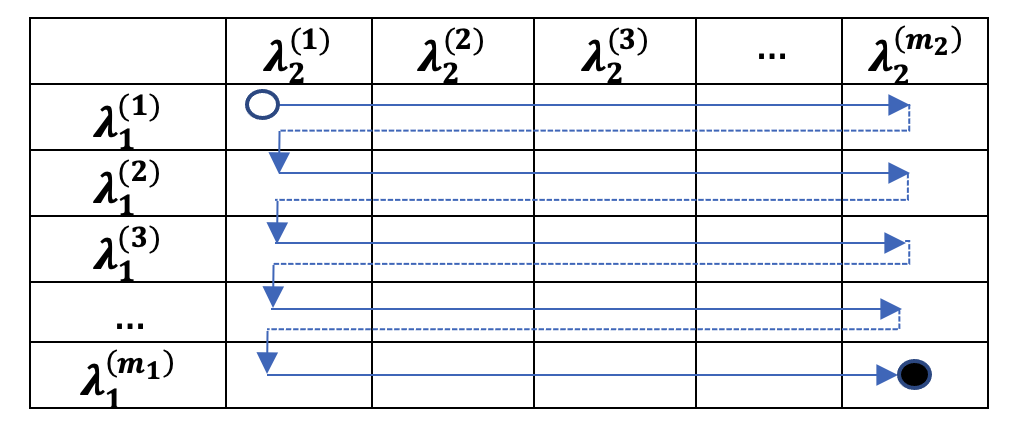
\includegraphics[scale=0.8]{2D-grid}
  \caption[Two-dimensional grid pathwise optimization]{
    Two-dimensional grid pathwise optimization.
  }
  \label{fig:2d}
\end{figure}

\subsection{Computation of diagonal elements of weight matrix}
\label{a.3}
Diagonal elements of weight matrix $\bm{W}$, the Hessian of log of Cox'x partial likelihood function, has the form 
\begin{displaymath}
w_i=\sum_{k\in C_i}\frac{d_k e^{\tilde{\eta}_i}}{\sum_{j\in R_i}e^{\tilde{\eta}_j}}-\sum_{k\in C_i}\frac{d_k (e^{\tilde{\eta}_i})^2}{(\sum_{j\in R_i}e^{\tilde{\eta}_j})^2}. 
\end{displaymath}
The two sums $\sum_{k\in C_i}$ and $\sum_{j\in R_i}$ both have $n$ elements, hence it is a $O(n^2)$ computation. However, if we notice the difference between $R_k$ and $R_{k+1}$ is the observations that are in $R_k$ but not in $R_{k+1}$, i.e., $\{j:t_k\leq y_j < t_{k+1}\}$, provided that the observed times $\bm{y}$ are sorted in non-decreasing order, then $\sum_{j\in R_k}e^{\tilde{\eta}_j}$ can be calculated as cumulative sums:
\begin{displaymath}
\sum_{j\in R_k} e^{\tilde{\eta}_j} =\sum_{j\in R_{k+1}} e^{\tilde{\eta}_j}+ \sum_{j\in R_k \& j\notin R_{k+1}} e^{\tilde{\eta}_j}.
\end{displaymath}
The same cumulative sum idea can be applied to $\sum_{k\in C_i}$: 
\begin{align*}
    \sum_{k\in C_{i+1}}\frac{d_k e^{\tilde{\eta}_i}}{\sum_{j\in R_i}e^{\tilde{\eta}_j}}&=\sum_{k\in C_i}\frac{d_k e^{\tilde{\eta}_i}}{\sum_{j\in R_i}e^{\tilde{\eta}_j}}+\sum_{k\in C_i\&k\notin c_{i+1}}\frac{d_k e^{\tilde{\eta}_i}}{\sum_{j\in R_i}e^{\tilde{\eta}_j}}, \\
    \sum_{k\in C_{i+1}}\frac{d_k (e^{\tilde{\eta}_i})^2}{(\sum_{j\in R_i}e^{\tilde{\eta}_j})^2}&=\sum_{k\in C_i}\frac{d_k (e^{\tilde{\eta}_i})^2}{(\sum_{j\in R_i}e^{\tilde{\eta}_j})^2}+ \sum_{k\in C_i\&k\notin c_{i+1}}\frac{d_k (e^{\tilde{\eta}_i})^2}{(\sum_{j\in R_i}e^{\tilde{\eta}_j})^2}.
\end{align*}
The equations above only calculate the sums once, and add at each sample index, which brings the computation cost down to linear time, $O(n)$. Considering sorting observed times as a data pre-processing procedure, the overall computation time for the weights is $O(n\log n)$. 


\subsection{Example codes for R package `xrnet'}
\label{a.4}

\section{Appendix for Chapter 3}
